\documentclass{article}

% if you need to pass options to natbib, use, e.g.:
%     \PassOptionsToPackage{numbers, compress}{natbib}
% before loading neurips_2020

% ready for submission
% \usepackage{neurips_2020}

% to compile a preprint version, e.g., for submission to arXiv, add add the
% [preprint] option:
%     \usepackage[preprint]{neurips_2020}

% to compile a camera-ready version, add the [final] option, e.g.:
%     \usepackage[final]{neurips_2020}

% to avoid loading the natbib package, add option nonatbib:
     \usepackage[nonatbib]{neurips_2020}

\usepackage[utf8]{inputenc} % allow utf-8 input
\usepackage[T1]{fontenc}    % use 8-bit T1 fonts
\usepackage{hyperref}       % hyperlinks
\usepackage{url}            % simple URL typesetting
\usepackage{booktabs}       % professional-quality tables
\usepackage{amsfonts}       % blackboard math symbols
\usepackage{nicefrac}       % compact symbols for 1/2, etc.
\usepackage{microtype}      % microtypography
\usepackage{graphicx,booktabs,multirow}

\title{Admission Data Prediction Using Machine Learning Methods}

% The \author macro works with any number of authors. There are two commands
% used to separate the names and addresses of multiple authors: \And and \AND.
%
% Using \And between authors leaves it to LaTeX to determine where to break the
% lines. Using \AND forces a line break at that point. So, if LaTeX puts 3 of 4
% authors names on the first line, and the last on the second line, try using
% \AND instead of \And before the third author name.

\author{
  David S.~Hippocampus\   thanks{Use footnote for providing further information
    about author (webpage, alternative address)---\emph{not} for acknowledging
    funding agencies.} \\
  Department of Computer Science\\
  Cranberry-Lemon University\\
  Pittsburgh, PA 15213 \\
  % examples of more authors
  % \And
  % Coauthor \\
  % Affiliation \\
  % Address \\
  % \texttt{email} \\
  % \AND
  % Coauthor \\
  % Affiliation \\
  % Address \\
  % \texttt{email} \\
  % \And
  % Coauthor \\
  % Affiliation \\
  % Address \\
  % \texttt{email} \\
  % \And
  % Coauthor \\
  % Affiliation \\
  % Address \\
  % \texttt{email} \\
}

\begin{document}

\maketitle

\begin{abstract}
  The 
\end{abstract}

\section{Introduction}

NeurIPS requires electronic submissions.  The electronic submission site is
\begin{center}
  \url{https://cmt3.research.microsoft.com/NeurIPS2020/}
\end{center}

Please read the instructions below carefully and follow them faithfully.

















\section{Methodology}
\label{gen_inst}
The dataset we chose is created for prediction of Graduate Admissions from an Indian perspective, which predicting admission from 7 important parameters with 500 students. The output is a number from 0 to 100, which represents the probably a student being admitted. Therefore, we consider it as a regression problem.

\subsection{Preprocessing}
Firstly, we do the data splitting process, we randomly divide 500 input data into three parts: 320 train data, 80 validation data, and 100 testing data.
Secondly, we do subset selection to find the best subset of 7 feature parameters. Based on the RSS loss of linear regression, we find out that the best subset is the total set, we do not need to filter any feature parameter.
Then, we normalize the input data before loading them into algorithm models.
Additionally, some algorithm may not support regression task, such as logistic regression, LDA, and Naive Bayes, so for these algorithm, we change the regression task into classification task by approximating the output number into 10 neighbor classes: 0, 10, 20, and so on.

\subsection{Algorithm}

In order to solve this problem, we considering both classification methods and regression methods. The original data is continuous and we will preprocessing it if we want to use classification methods.

\textbf{Least square} Fit a linear model with coefficients $w = (w_1, ..., w_p)$ to minimize the sum of squared residuals between the actual observed data and the predicted data (estimated values) of the data set: $min_w ||Xw-y||_2^2$.\\
\textbf{Ridge regression} Ridge regression solves some problems of ordinary least squares by penalizing the size of the coefficients. What minimizes the ridge coefficiet is the sum of squared residuals with penalties: $min_w ||Xw-y||_2^2+\alpha ||w||_2^2$.\\
\textbf{Lasso regression} Lasso regression consists of a linear model with regular terms of $l_1$-norm. Its minimized objective function is: $min_w \frac{1}{2n_{samples}} ||Xw-y||_2^2+\alpha ||w||_1$.\\
\textbf{Knn} Knn is also a regression method, it is used when the data labels are continuous variables rather than discrete variables. The label assigned to the query point is calculated from the average of its nearest neighbor labels.\\
\textbf{Decision tree} The nearest neighbor regression is used when the data labels are continuous variables rather than discrete variables. The label assigned to the query point is calculated from the average of its nearest neighbor labels.\\
\textbf{SVM}It is very efficient in high-dimensional space, and different kernel functions have a one-to-one correspondence with specific decision functions. Common kernels are already provided, and custom kernels can also be specified.\\
\textbf{Boosting} The goal of the boosting method is to combine the prediction results of multiple base estimators constructed using a given learning algorithm to obtain better generalization ability/robustness than a single estimator. We mainly focus on Random Forest and AdaBoost.\\
\textbf{LDA} This is a classification method. It is derived from simple probability models, and these models can be obtained by Bayes' theorem for the relevant distribution $P(X|y=k)$ of each category k.
\textbf{Naïve Bayes} This is a classification method. Naive Bayes methods are a set of supervised learning algorithms based on applying Bayes’ theorem with the “naive” assumption of conditional independence between every pair of features given the value of the class variable.\\
\textbf{Logistic} This is a classification method. Logistic regression is a generalized linear model, so it has many similarities with multiple linear regression analysis. Their model form is basically the same. It gets dependent variable value by logistic function.

\section{Experiment}
\label{headings}

\subsection{Preprocessing}

In the preprocessing process, after splitting data into training, validation and testing data, and before normalization, we do subset selection to find the best subset of 7 feature parameters. During subset selection, For each $s \in 0, 1, ... , p$, find the subset in size of $s$ that gives lowest RSS, and use cross-validation to esitimate prediction error and select $s$. Then, we can select the optimal variables. The result is showed below. We can learn from the result that the best subset is the total set, we do not need to filter any feature parameter. In addition, it is quite friedly for us to use the moethod to selection the best subset, since it need a lot of computation and a lot of time when $p$ is too large, but our $p$ is $7$, and the dataset is small, so the running time is not too long.

\begin{figure}[h]
	\centering
	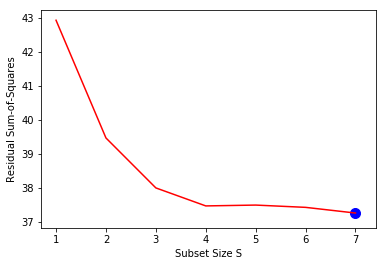
\includegraphics[width=6.5cm]{preprocessing.jpg}
	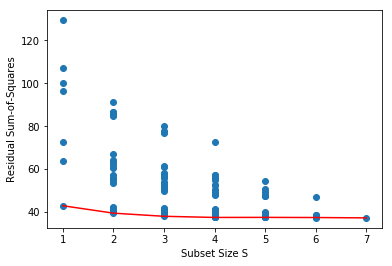
\includegraphics[width=6.5cm]{preprocessing2.jpg}
	\caption{Subset Selection Result.}
\end{figure}

\subsection{Algorithm}


\subsubsection{Regression}
First, we use regression algorithm to fit the admission rate. We use without shrinkage, lasso and ridge models to find the best model, by optimizing the parameter alpha through the analysis of RSS error. Alpha indicates the degree of shrinkage. When alpha approaches 1, it indicates that the degree of shrinkage reaches its maximum; when alpha approaches 0, it indicates that there is no shrinkage.
The RSS of the three methods varies with alpha are shown as follows. It can be seen that the smallest RSS is at lasso regression, and the alpha at this time is 0.3419, the accuracy is 0.8706.
\begin{figure}[h]
	\centering
	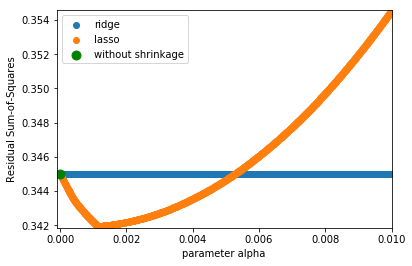
\includegraphics[width=6.5cm]{linear_regression.jpg}
	\caption{Subset Selection Result.}
\end{figure}

\subsubsection{Decision Tree}
In decision tree algorithm, we find the optimal model by finding at which depth we will get the lowest residual sum-of-squares in validation set.
From Figure 2 we can know that we can get the lowest residual sum-of-squares at $depth = 4$, and the RSS value is $0.4518$. The accuracy of this method is $0.8386$.
\begin{figure}[h]
	\centering
	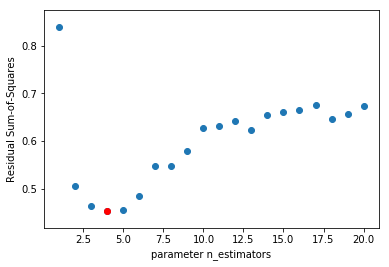
\includegraphics[width=6.5cm]{decision_tree.jpg}
	\caption{Subset Selection Result.}
\end{figure}

\subsubsection{KNN}
Using KNN regression, we need to find the optimal $k$ value. We want to find at which $k$ value we will get the lowest residual sum-of-squares in validation set.
\begin{figure}[h]
	\centering
	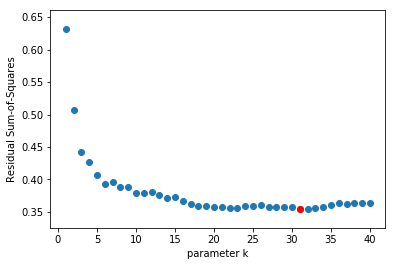
\includegraphics[width=6.5cm]{knn.jpg}
	\caption{Knn Result.}
\end{figure}
\\From Figure 2 we can know that we can get the lowest residual sum-of-squares at $k=31$, and the RSS value is $0.3546$. The accuracy of this method is $0.8706$.



\subsubsection{SVM}
In SVM regression method, we can apply different kernel on it. The min error without any kernel is $0.5596$.
\begin{itemize}
	\item \textbf{rbf kernel}: We will find the lowest residual sum-of-squares in validation set at $gamma =5.0351e-05$, and the RSS value is $0.4495$. The accuracy of this method is $0.6179$.
	\begin{figure}[h]
		\centering
		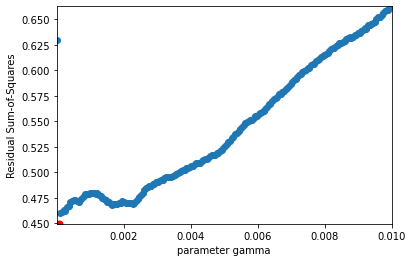
\includegraphics[width=6.5cm]{svm1.jpg}
		\caption{rbf kernel}
	\end{figure}
	\item \textbf{linear kernel}: We will find the lowest residual sum-of-squares in validation set at $C=0.0918$, and the RSS value is $0.4476$. The accuracy of this method is $0.6221$.
	\begin{figure}[h]
		\centering
		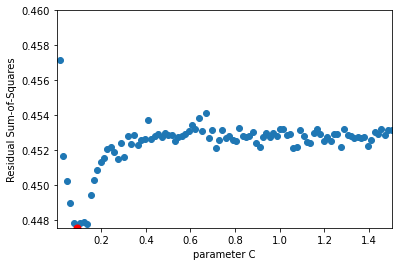
\includegraphics[width=6.5cm]{svm2.jpg}
		\caption{linear kernel}
	\end{figure}
	\item \textbf{poly kernel}: We will find the lowest residual sum-of-squares in validation set at $degree=1$, and the RSS value is $0.4532$. The accuracy of this method is $0.6211$.
\end{itemize}

\subsubsection{AdaBoost}
When we using AdaBoost method, we are using a lot of weak estimators to regress this problem. So we want to find the optimal number of the weak estimators.
\\We will find the lowest residual sum-of-squares in validation set at the $n\_estimators =10$, and the RSS value is $0.3951$. The accuracy of this method is $0.6836$.
\begin{figure}[h]
	\centering
	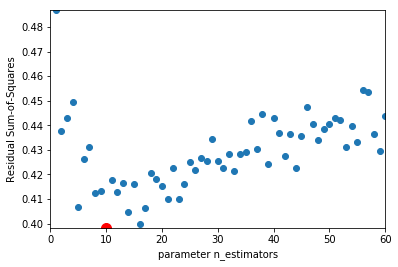
\includegraphics[width=6.5cm]{adaboost1.jpg}
	\caption{AdaBoost: estimator number and RSS}
\end{figure}
\\At the same time, we realized that the running time may have some relation with the number of the weak estimators, and then we record the running time of this method with different number of the weak estimators.
\begin{figure}[h]
	\centering
	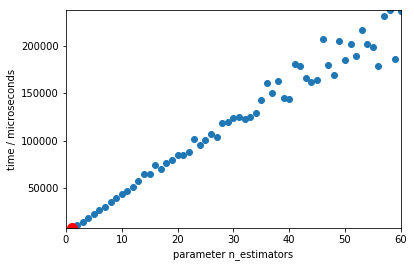
\includegraphics[width=6.5cm]{adaboost2.jpg}
	\caption{AdaBoost: estimator number and RSS}
\end{figure}
\\The min time is $11035$ microseconds at $n\_estimators =1$, and the running time increases as the number of the weak estimators increases. We can get the conclusion that the optimal RSS may not correspond with the shortest running time.

\subsubsection{Random Forest}
In random forest algorithm, we need to find the optimal model by finding the optimal n\_estimators and optimal depth, by get the lowest residual sum-of-squares in validation set.\\
Firstly, we choose best n\_estimators by running model with diffirent n\_estimators and choose the best. But during this process, we find out as n\_estimators increase, the time that cost to run the algorithm increase linearly, so its not elegant to choose large n\_estimators. After finding the optimal n\_estimators, we start finding the optimal depth with optimal n\_estimators, the thild figure in Figure 4 shows that at $depth = 4$, the validation error reach maximum. Also, the model start overfitting at around $depth = 3$.\\
From Figure 3 we can know that we can get the lowest residual sum-of-squares in the validation set at $depth = 4$, $n\_estimators = 13$, and the RSS value is $0.3797$. The accuracy of this method is $0.8303$.
\begin{figure}[h]
	\centering
	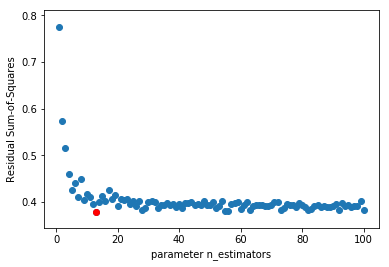
\includegraphics[width=6.2cm]{random_forest1.jpg}
	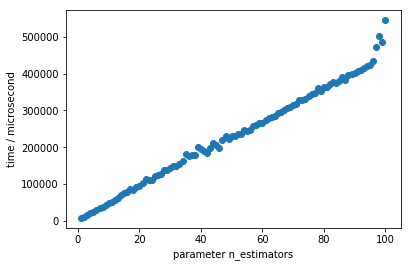
\includegraphics[width=6.5cm]{random_forest2.jpg}
	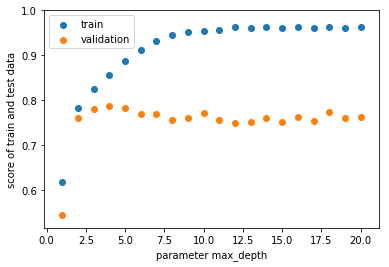
\includegraphics[width=6.5cm]{random_forest3.jpg}
	\caption{Subset Selection Result.}
\end{figure}


\subsubsection{Other}
Besides the regression method above, we also use some classification methods to solve this problem.
\begin{itemize}
	\item \textbf{Logistic} When we try different penalty function, we find that $l_1$ function is a little bit better than $l_2$. The lowest residual sum-of-squares in validation set is $0.7880$, and the accuracy is $0.4810$.
	\item \textbf{Naïve Bayes} Comparing Gaussian NB and Bernoulli NB, we find that Gaussian NB has better effect. The lowest residual sum-of-squares in validation set is $0.7$, and the accuracy is $0.5952$.
	\item \textbf{LDA} The LDA method with default solver $svd$ can reach the accuracy $0.5833$, and the lowest residual sum-of-squares in validation set is $0.5440$.
\end{itemize}



\begin{table}
	\caption{Sample table title}
	\label{sample-table}
	\centering
	\begin{tabular}{ccccccccc}
		\toprule
		Algorithm     & RSS error     & Accuracy \\
		\midrule
		regression(Lasso) & \textbf{0.3419}  & \textbf{87.057\%}     \\
		KNN     & \textbf{0.3546} & 81.570\%     \\
		Decision Tree     & 0.4518       & \textbf{83.863\%}  \\
		SVM(Linear)     & 0.4476      & 62.206\%  \\
		AdoBoost     & 0.3982       & 69.178\% \\
		Random Forest    & \textbf{0.3797}       & \textbf{83.029\%}  \\
		LDA   & 0.5440       & 58.333\%  \\
		Naive Bayes(Gaussian)    & 0.7000       & 59.5238\%  \\
		Logistic(l1-penalty)    & 0.7880       & 48.0952\%  \\
		\bottomrule
	\end{tabular}
\end{table}










\section{Conclusion}
\label{others}

These instructions apply to everyone.

\subsection{Citations within the text}

The \verb+natbib+ package will be loaded for you by default.  Citations may be
author/year or numeric, as long as you maintain internal consistency.  As to the
format of the references themselves, any style is acceptable as long as it is
used consistently.

The documentation for \verb+natbib+ may be found at
\begin{center}
  \url{http://mirrors.ctan.org/macros/latex/contrib/natbib/natnotes.pdf}
\end{center}
Of note is the command \verb+\citet+, which produces citations appropriate for
use in inline text.  For example,
\begin{verbatim}
   \citet{hasselmo} investigated\dots
\end{verbatim}
produces
\begin{quote}
  Hasselmo, et al.\ (1995) investigated\dots
\end{quote}

If you wish to load the \verb+natbib+ package with options, you may add the
following before loading the \verb+neurips_2020+ package:
\begin{verbatim}
   \PassOptionsToPackage{options}{natbib}
\end{verbatim}

If \verb+natbib+ clashes with another package you load, you can add the optional
argument \verb+nonatbib+ when loading the style file:
\begin{verbatim}
   \usepackage[nonatbib]{neurips_2020}
\end{verbatim}

As submission is double blind, refer to your own published work in the third
person. That is, use ``In the previous work of Jones et al.\ [4],'' not ``In our
previous work [4].'' If you cite your other papers that are not widely available
(e.g., a journal paper under review), use anonymous author names in the
citation, e.g., an author of the form ``A.\ Anonymous.''

\subsection{Footnotes}

Footnotes should be used sparingly.  If you do require a footnote, indicate
footnotes with a number\footnote{Sample of the first footnote.} in the
text. Place the footnotes at the bottom of the page on which they appear.
Precede the footnote with a horizontal rule of 2~inches (12~picas).

Note that footnotes are properly typeset \emph{after} punctuation
marks.\footnote{As in this example.}

\subsection{Figures}

\begin{figure}
  \centering
  \fbox{\rule[-.5cm]{0cm}{4cm} \rule[-.5cm]{4cm}{0cm}}
  \caption{Sample figure caption.}
\end{figure}

All artwork must be neat, clean, and legible. Lines should be dark enough for
purposes of reproduction. The figure number and caption always appear after the
figure. Place one line space before the figure caption and one line space after
the figure. The figure caption should be lower case (except for first word and
proper nouns); figures are numbered consecutively.

You may use color figures.  However, it is best for the figure captions and the
paper body to be legible if the paper is printed in either black/white or in
color.

\subsection{Tables}

All tables must be centered, neat, clean and legible.  The table number and
title always appear before the table.  See Table~\ref{sample-table}.

Place one line space before the table title, one line space after the
table title, and one line space after the table. The table title must
be lower case (except for first word and proper nouns); tables are
numbered consecutively.

Note that publication-quality tables \emph{do not contain vertical rules.} We
strongly suggest the use of the \verb+booktabs+ package, which allows for
typesetting high-quality, professional tables:
\begin{center}
  \url{https://www.ctan.org/pkg/booktabs}
\end{center}
This package was used to typeset Table~\ref{sample-table}.


\section{Final instructions}

Do not change any aspects of the formatting parameters in the style files.  In
particular, do not modify the width or length of the rectangle the text should
fit into, and do not change font sizes (except perhaps in the
\textbf{References} section; see below). Please note that pages should be
numbered.

\section{Preparing PDF files}

Please prepare submission files with paper size ``US Letter,'' and not, for
example, ``A4.''

Fonts were the main cause of problems in the past years. Your PDF file must only
contain Type 1 or Embedded TrueType fonts. Here are a few instructions to
achieve this.

\begin{itemize}

\item You should directly generate PDF files using \verb+pdflatex+.

\item You can check which fonts a PDF files uses.  In Acrobat Reader, select the
  menu Files$>$Document Properties$>$Fonts and select Show All Fonts. You can
  also use the program \verb+pdffonts+ which comes with \verb+xpdf+ and is
  available out-of-the-box on most Linux machines.

\item The IEEE has recommendations for generating PDF files whose fonts are also
  acceptable for NeurIPS. Please see
  \url{http://www.emfield.org/icuwb2010/downloads/IEEE-PDF-SpecV32.pdf}

\item \verb+xfig+ "patterned" shapes are implemented with bitmap fonts.  Use
  "solid" shapes instead.

\item The \verb+\bbold+ package almost always uses bitmap fonts.  You should use
  the equivalent AMS Fonts:
\begin{verbatim}
   \usepackage{amsfonts}
\end{verbatim}
followed by, e.g., \verb+\mathbb{R}+, \verb+\mathbb{N}+, or \verb+\mathbb{C}+
for $\mathbb{R}$, $\mathbb{N}$ or $\mathbb{C}$.  You can also use the following
workaround for reals, natural and complex:
\begin{verbatim}
   \newcommand{\RR}{I\!\!R} %real numbers
   \newcommand{\Nat}{I\!\!N} %natural numbers
   \newcommand{\CC}{I\!\!\!\!C} %complex numbers
\end{verbatim}
Note that \verb+amsfonts+ is automatically loaded by the \verb+amssymb+ package.

\end{itemize}

If your file contains type 3 fonts or non embedded TrueType fonts, we will ask
you to fix it.

\subsection{Margins in \LaTeX{}}

Most of the margin problems come from figures positioned by hand using
\verb+\special+ or other commands. We suggest using the command
\verb+\includegraphics+ from the \verb+graphicx+ package. Always specify the
figure width as a multiple of the line width as in the example below:
\begin{verbatim}
   \usepackage[pdftex]{graphicx} ...
   \includegraphics[width=0.8\linewidth]{myfile.pdf}
\end{verbatim}
See Section 4.4 in the graphics bundle documentation
(\url{http://mirrors.ctan.org/macros/latex/required/graphics/grfguide.pdf})

A number of width problems arise when \LaTeX{} cannot properly hyphenate a
line. Please give LaTeX hyphenation hints using the \verb+\-+ command when
necessary.



\begin{ack}
Use unnumbered first level headings for the acknowledgments. All acknowledgments
go at the end of the paper before the list of references. Moreover, you are required to declare 
funding (financial activities supporting the submitted work) and competing interests (related financial activities outside the submitted work). 
More information about this disclosure can be found at: \url{https://neurips.cc/Conferences/2020/PaperInformation/FundingDisclosure}.


Do {\bf not} include this section in the anonymized submission, only in the final paper. You can use the \texttt{ack} environment provided in the style file to autmoatically hide this section in the anonymized submission.
\end{ack}

\section*{References}

References follow the acknowledgments. Use unnumbered first-level heading for
the references. Any choice of citation style is acceptable as long as you are
consistent. It is permissible to reduce the font size to \verb+small+ (9 point)
when listing the references.
{\bf Note that the Reference section does not count towards the eight pages of content that are allowed.}
\medskip

\small

[1] Alexander, J.A.\ \& Mozer, M.C.\ (1995) Template-based algorithms for
connectionist rule extraction. In G.\ Tesauro, D.S.\ Touretzky and T.K.\ Leen
(eds.), {\it Advances in Neural Information Processing Systems 7},
pp.\ 609--616. Cambridge, MA: MIT Press.

[2] Bower, J.M.\ \& Beeman, D.\ (1995) {\it The Book of GENESIS: Exploring
  Realistic Neural Models with the GEneral NEural SImulation System.}  New York:
TELOS/Springer--Verlag.

[3] Hasselmo, M.E., Schnell, E.\ \& Barkai, E.\ (1995) Dynamics of learning and
recall at excitatory recurrent synapses and cholinergic modulation in rat
hippocampal region CA3. {\it Journal of Neuroscience} {\bf 15}(7):5249-5262.

\end{document}
